\section{Medical background}
The brain scans in the BraTS\cite{menze2015multimodal} 2018 dataset were made with MRI scanners\cite{mriscanner}.
The brain consists mostly of water. Water molecules contain two hydrogen molecules, each of which has one proton. A proton spins in a specific direction. When a strong magnet is applied to a proton, the proton starts to spin in the same direction as the magnet. 

A MRI scanner can generate a very precise and targeted magnetic field. When the magnet is deactivated, the protons go back into their resting position. Depending on the material a proton is part of (gray matter, necrotic tissue, cerebrospinal fluid  etc.), the resting position of the proton is different and a different amount of energy is released when the proton returns to its resting position. This energy is measured by the MRI scanner and visualized as a scan. MRI scanners go trough the brain in layers and generate a 2D image of every layer called a slice. The output of an MRI scanner is therefore a 3D volume.

\subsection{Slice modalities}
The BraTS dataset contains four different slice types, called modalities. These types are generated by specific settings of the MRI machine and by inserting a contrast enhancing fluid into the brain of the patient.

\subsubsection{T1}
For the T1 modality scan, the MRI machine measures the vertical movement of the protons when returning to their resting position. This modality mainly highlights fat and therefore contrast between fat and other tissues, e.g. nerve roots\cite{mriquora}. This modality only faintly shows tumor tissues, as seen in Figure \ref{medical_background_t1}.

\begin{figure}[H]
    \centering
    \begin{subfigure}{.5\textwidth}
        \centering
        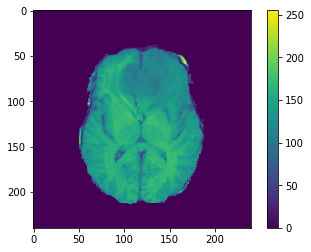
\includegraphics[width=\linewidth]{chapters/04_segmentation/images/medical_background/t1.png}
        \caption{T1 modality}
    \end{subfigure}%
    \begin{subfigure}{.5\textwidth}
        \centering
        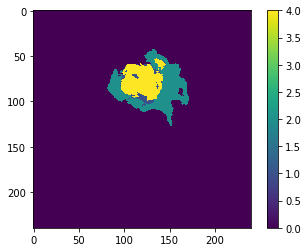
\includegraphics[width=\linewidth]{chapters/04_segmentation/images/medical_background/tumor.png}
        \caption{Tumor ground truth}
    \end{subfigure}
    \caption{The left image shows the T1 modality of a slice. There is only a small correlation with the gadolinium-enhancing tumor tissue in the tumor ground truth (yellow, value 4) and also cerebrospinal fluid in the center lower half of the image.}
    \label{medical_background_t1}
\end{figure}



\subsubsection{T2}
The T2 modality measures the horizontal movement of the protons returning to their resting position. This modality highlights water, e.g. cerebrospinal fluid, but also edema tissue as seen in Figure \ref{medical_background_t2}.
\begin{figure}[H]
    \centering
    \begin{subfigure}{.5\textwidth}
        \centering
        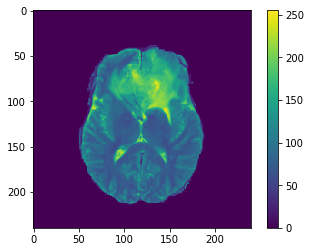
\includegraphics[width=\linewidth]{chapters/04_segmentation/images/medical_background/t2.png}
        \caption{T2 modality}
    \end{subfigure}%
    \begin{subfigure}{.5\textwidth}
        \centering
        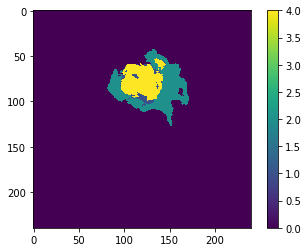
\includegraphics[width=\linewidth]{chapters/04_segmentation/images/medical_background/tumor.png}
        \caption{Tumor ground truth}
    \end{subfigure}
    \caption{The left image shows the T2 modality of a slice. Clearly visible is the edema of the tumor ground truth (turquoise, value 2.0).}
    \label{medical_background_t2}
\end{figure}




\subsubsection{T1 contrast enhanced}
Gadolinium is a chemical compound given to the patient during MRI scans that highlights areas of inflammation.
The scanner itself has the same setting as with a non-contrast enhanced T1 scan. The inflammed gadolinium enhanced tumor is clearly visible in Figure \ref{medical_background_t1ce}.

\begin{figure}[H]
    \centering
    \begin{subfigure}{.5\textwidth}
        \centering
        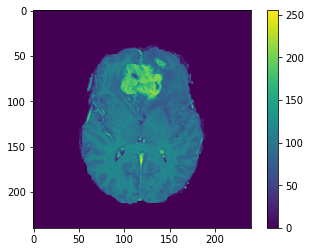
\includegraphics[width=\linewidth]{chapters/04_segmentation/images/medical_background/t1ce.png}
        \caption{T1 contrast enhanced}
    \end{subfigure}%
    \begin{subfigure}{.5\textwidth}
        \centering
        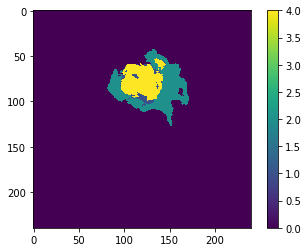
\includegraphics[width=\linewidth]{chapters/04_segmentation/images/medical_background/tumor.png}
        \caption{Tumor ground truth}
    \end{subfigure}
    \caption{The left image shows the T1 contrast enhanced modality of a slice. Clearly visible is the gadolinium enhanced tumor (yellow, value 4.0).}
    \label{medical_background_t1ce}
\end{figure}



\subsubsection{T2 FLAIR}
T2 FLAIR (Fluid-Attenuated Inversion Recovery) \cite{mribasics} is similar to the T2 modality. The difference to T2 is the much longer time between magnet pulses by the MRI machine.
The images are similar to the T2 images, but cerebrospinal fluid is much darker and actual tumor tissue is brighter, as seen in Figure \ref{medical_background_flair}. The disadvantage
of this method is the reduced sharpness of the image.

\begin{figure}[H]
    \centering
    \begin{subfigure}{.5\textwidth}
        \centering
        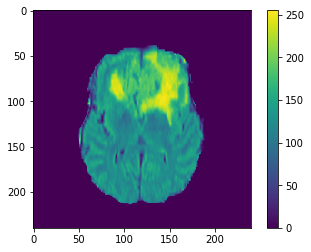
\includegraphics[width=\linewidth]{chapters/04_segmentation/images/medical_background/flair.png}
        \caption{FLAIR Modality}
    \end{subfigure}%
    \begin{subfigure}{.5\textwidth}
        \centering
        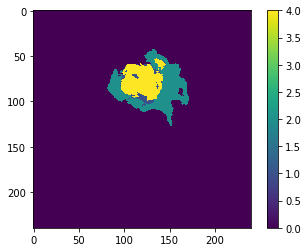
\includegraphics[width=\linewidth]{chapters/04_segmentation/images/medical_background/tumor.png}
        \caption{Tumor ground truth}
    \end{subfigure}
    \caption{The left image shows the FLAIR modality of a slice. Clearly visible is the edema of the tumor ground truth (turquoise, value 2.0), but also the other parts of the tumor.
    In comparison to T2, the cerebrospinal fluid in the lower half of the brain is almost black.}
    \label{medical_background_flair}
\end{figure}
